\documentclass{beamer}
\usepackage{amsfonts,amsmath,oldgerm}
\usepackage{multicol, graphicx, caption}
\usepackage{pgfplots}
\usepackage{tikz}
\usetheme{sintef}

\newcommand{\testcolor}[1]{\colorbox{#1}{\textcolor{#1}{test}}~\texttt{#1}}

\usefonttheme[onlymath]{serif}

\titlebackground*{images/background}

\newcommand{\hrefcol}[2]{\textcolor{cyan}{\href{#1}{#2}}}

\title{Neural Networks}
% \subtitle{Using \LaTeX\ to prepare slides}
\author{\href{mailto:olivertemple@exe-coll.ac.uk}{Oliver Temple}}
\date{March 8, 2022}

\begin{document}
\maketitle

% intro - "What is a neural network?..."  My name is Oliver Temple and I am here to talk to you about neural networks. You may well have heard the term neural network before, you may even know what they are, but I am going to start from the beginning and explain what a neural network is and how one of the most basic models works.

% Slide 1 - A neural network is a complex computational model that can be used to perform a wide range of tasks from image recognition to classification and prediction. They are constructed from interconnected neurons organized into layers, as shown in this figure.

\begin{frame}{What a Neural Network Is}
    \begin{center}
        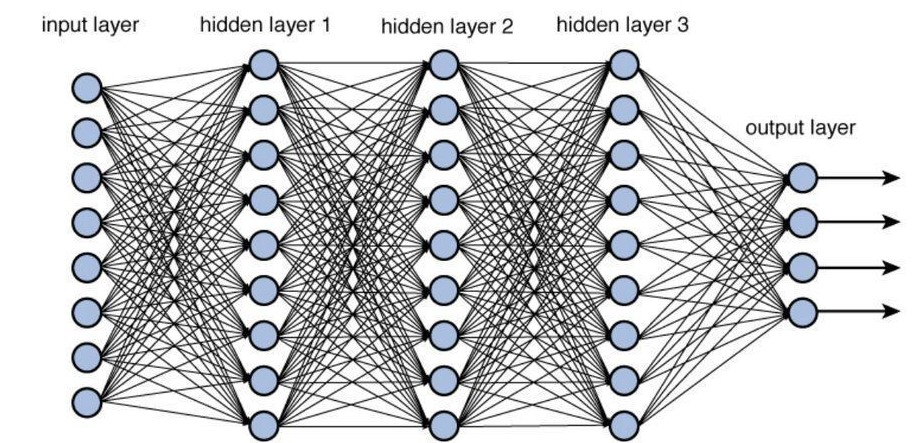
\includegraphics[width=\textwidth]{images/neural_network}
        \captionof{figure}{Representation of a neural network}
    \end{center}
\end{frame}



% Slide 2 - Neural networks are able to be used for such a wide variety of uses as there are so many variations of how the neurons can be organized and connected to each other. Some of the most common models are the perceptron, the feed forward neural network and the multi-layer neural network. and biases of each layer.
\begin{frame}{Types of Neural Network}
    \begin{itemize}
        \item Perceptron
        \item Feed Forward Neural Network
        \item Multi-layer Perceptron
    \end{itemize}
\end{frame}

%Slide 3 - A perceptron, often referred to as a neuron, is one of the simplest and oldest forms of neural networks. It accepts multiple inputs ranging from 0 to 1, and uses the weight that each connection has to calculate the output by taking the vector dot product of the inputs and the weights. The bias is then added and the result is then passed through an activation function to give the output. 
\begin{frame}{Types of Neural Network}{Perceptron}
\begin{multicols}{2}
    \begin{equation}
        \textbf{y} = \sigma(\textbf{W}\cdot\textbf{x} + b)
    \end{equation}
    Where $\textbf{y}$ is the output, $\textbf{W}$ is a vector of the weights, $\textbf{x}$ is a vector of the inputs, $b$ is the bias and $\sigma$ is the activation function.
    \begin{center}
        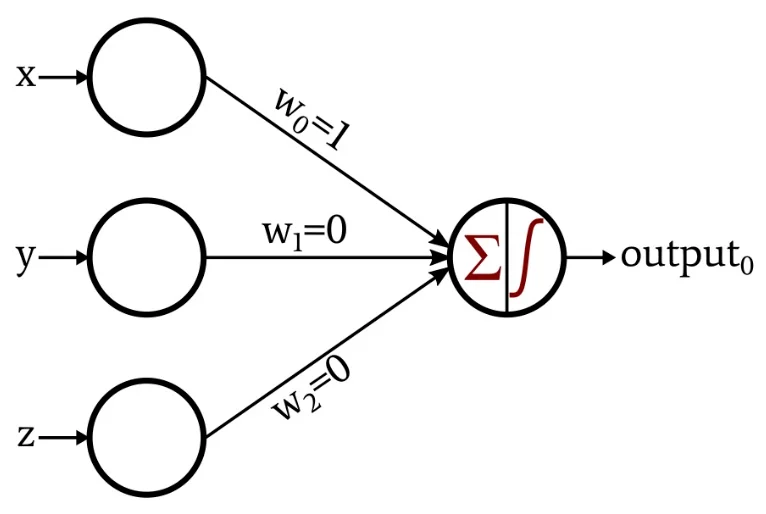
\includegraphics[width=0.5\textwidth]{images/perceptron}
        \captionof{figure}{Perceptron}
    \end{center}
\end{multicols}
\end{frame}

%Slide 4 - A feed forward neural network is a neural network that is constructed from interconnected layers of neurons. Each neuron in a layer is connected to every neuron in the previous layer and the output of the previous layer is used as the input to the next layer. The data only travels in one direction, meaning that it cannot be trained, so is only useful for linear classification. The output of the nth layer is calculated by taking the dot product of the weight matrix and the input vector and adding the bias. The result is then passed through an activation function to give the output.
\begin{frame}{Types of Neural Network}{Feed Forward Neural Network}
\begin{multicols}{2}
    \begin{equation}
        \textbf{y}_n=\sigma{(\textbf{W}_n\cdot\textbf{y}_{n-1} + \textbf{b}_n)}
    \end{equation}
    Where $\textbf{y}_n$ is the output vector of the nth layer, $\textbf{W}_n$ is the weight matrix of the nth layer, $\textbf{y}_{n-1}$ is the output vector of the previous layer, $\textbf{b}_n$ is the bias vector of the nth layer, and $\sigma$ is the activation function.
    \begin{center}
        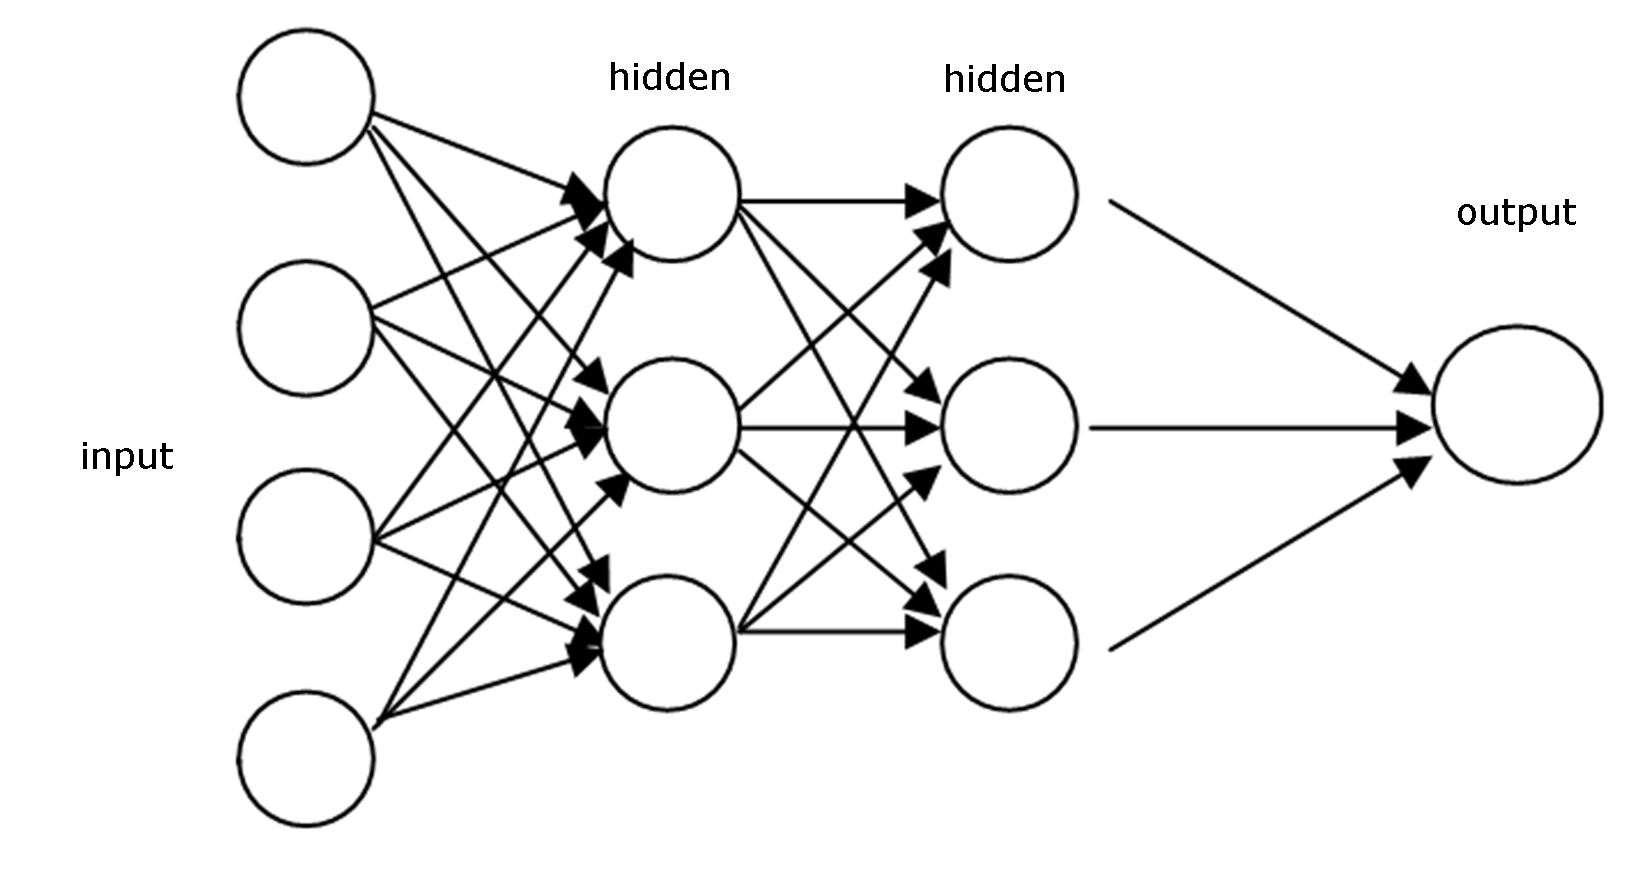
\includegraphics[width=0.5\textwidth]{images/feed forward}
        \captionof{figure}{Feed Forward Neural Network}
    \end{center}
\end{multicols}
\end{frame}

\begin{frame}{Types of Neural Network}{Multi-layer Perceptron}
    \begin{equation}
        \textbf{y}_n=\sigma{(\textbf{W}_n\cdot\textbf{y}_{n-1} + \textbf{b}_n)}
    \end{equation}
    Where $\textbf{y}_n$ is the output vector of the nth layer, $\textbf{W}_n$ is the weight matrix of the nth layer, $\textbf{y}_{n-1}$ is the output vector of the previous layer, $\textbf{b}_n$ is the bias vector of the nth layer, and $\sigma$ is the activation function.
\end{frame}


% At its core, a neural network is a collection of neurons, formed into layers, that are all interconnected.
% Each neuron has its own bias and each connection has its own weight.
% These parameters are what determine the output of the network.
\begin{frame}{How Neural Networks Work}
    \begin{itemize}
        \item Collection of interconnected neurons
        \item Each neuron has a bias
        \item Each connection has a weight
    \end{itemize}
\end{frame}

% The structure of the network is the first thing that must be defined.
% The input layer must consist of the same number of neurons as there are data points (e.g. one neuron per pixel in an image), and the output layer must consist of the same number of neurons as there are classification labels (the total number of outputs).
% There can be any number of hidden layers, which can have any number of neurons.
%  The size and number of hidden layers should be varied to determine what gives the best results.
\begin{frame}{How Neural Networks Work}{Structure}
    \begin{itemize}
        \item Input Layer
        \item Output Layer
        \item Hidden Layers
    \end{itemize}
\end{frame}

% The purpose of forward propagation is to get an output (or prediction) from our neural network.
% To calculate it we use the vector dot product of the inputs and the weights, add the bias and then apply the activation function, as shown in this equation
\begin{frame}{How Neural Networks Work}{Forward Propagation}
    \begin{itemize}
        \item Inputs are passed through the network to get a prediction
        \item $\textbf{y}_n=\sigma{(\textbf{W}_n\cdot\textbf{y}_{n-1} + \textbf{b}_n)}$
        \item Where $\textbf{y}_n$ is the output vector of the nth layer, $\textbf{W}_n$ is the weight matrix of the nth layer, $\textbf{y}_{n-1}$ is the output vector of the previous layer, $\textbf{b}_n$ is the bias vector of the nth layer, and $\sigma$ is the activation function.
    \end{itemize}
\end{frame}

% The activation function is applied to the output of each neuron before it is inputted into to the next layer.
% The purpose of an activation function is to prevent the input from being too high or too low, and to add some non-linearity to the network.
% There are many different activation functions to choose from, but some of the more common ones are sigmoid, than, relu and leaky relu. 
\begin{frame}{How Neural Networks Work}{Activation Functions}
    \begin{itemize}
        \item Sigmoid
        \item Tanh
        \item ReLU
        \item Leaky ReLU
    \end{itemize}
\end{frame}

% The sigmoid function, shown in this equation, takes any input, x, and translates it to a value between 0 and 1.
\begin{frame}{Activation Functions}{Sigmoid}
    \begin{multicols}{2}
        \begin{equation}
            \sigma(x)=\frac{1}{1+e^{-x}}
        \end{equation}
        \begin{center}
            \resizebox{0.5\textwidth}{!}{
                \begin{tikzpicture}
                    \begin{axis}[axis x line=bottom, axis y line=middle, xmin=-6, xmax=6, xlabel={$x$}, ylabel={$\sigma(x)$}]
                    \addplot[color=red]{1/(1+exp(-x))};
                    \end{axis}
                \end{tikzpicture}
            }
        \end{center}
    \end{multicols}
\end{frame}

% Similar to the sigmoid function, the than function, shown here, takes any input, x, and translates it to a value between -1 and 1.
\begin{frame}{Activation Functions}{Tanh}
    \begin{multicols}{2}
        \begin{equation}
            \tanh(x)=\frac{e^x-e^{-x}}{e^x+e^{-x}}
        \end{equation}
        \begin{center}
            \resizebox{0.5\textwidth}{!}{
                \begin{tikzpicture}
                    \begin{axis}[axis x line=bottom, axis y line=middle, xmin=-6, xmax=6, xlabel={$x$}, ylabel={$\tanh(x)$}]
                    \addplot[color=red]{tanh(x)};
                    \end{axis}
                \end{tikzpicture}
            }
        \end{center}
    \end{multicols}
\end{frame}

% Unlike the sigmoid function and the than function, the relu function takes any input, x, and if it is negative, returns 0 otherwise it returns x (the input).
\begin{frame}{Activation Functions}{ReLU}
    \begin{multicols}{2}
        \begin{equation}
            \text{ReLU}(x)=\max(0,x)
        \end{equation}
        \begin{center}
            \resizebox{0.5\textwidth}{!}{
                \begin{tikzpicture}
                    \begin{axis}[axis x line=bottom, axis y line=middle, xmin=-6, xmax=6, xlabel={$x$}, ylabel={$\text{R}(x)$}]
                    \addplot[color=red]{max(0,x)};
                    \end{axis}
                \end{tikzpicture}
            }
        \end{center}
    \end{multicols}
\end{frame}

% Leaky relu is much like the relu function, but it return 0.1 times the input for negative inputs.
\begin{frame}{Activation Functions}{leaky ReLU}
    \begin{multicols}{2}
        \begin{equation}
            \text{Leaky ReLU}(x) = \max(0.1x,x)
        \end{equation}
        \begin{center}
            \resizebox{0.5\textwidth}{!}{
                \begin{tikzpicture}
                    \begin{axis}[axis x line=middle, axis y line=middle, xmin=-6, xmax=6, xlabel={$x$}, ylabel={$\text{LR}(x)$}]
                    \addplot[color=red]{max(0.1*x,x)};
                    \end{axis}
                \end{tikzpicture}
            }
        \end{center}
    \end{multicols}
\end{frame}

% The loss function is used to calculate how good a model is.
% In order to calculate the loss, we need the output of our network, and the expected output.
% Similar to activation functions, there are many different loss functions to choose from.
% Two of the most common ones are mean squared error and cross entropy loss.
\begin{frame}{How Neural Networks Work}{Loss Functions}
    \begin{itemize}
        \item Mean Squared Error (MSE)
        \item Cross Entropy Loss (or Log Loss)
    \end{itemize}
\end{frame}

% The mean squared loss function, shown below, is calculated as the average of the squared difference between the predicted output and the expected output.
\begin{frame}{Loss Functions}{Mean Squared Error}
    \begin{equation}
        \text(MSE) = \frac{1}{n}\sum_{i=1}^{n}(\hat{y}_i-y_i)^2
    \end{equation}
    Where $n$ is the number if sample, $y_i$ is the desired output of the network and $\hat{y}_i$ is the actual output of the network.
\end{frame}

% Cross entropy loss, often called log loss, is a loss function that is used for more complex models.
% Each predicted output is compared to the desired output nd the score is calculated that penalizes the output based in the difference between the two.
% Tbe penalty is logarithmic, meaning a smaller score fore smaller differences, and a larger score for larger differences. It is calculated by taking the negative of the average of the predicted output and the logarithm of the output.
\begin{frame}{Loss Functions}{Cross Entropy Loss}
    \begin{equation}
        \text(CEL) = -\frac{1}{n}\sum_{i=1}^{n}(y_i\times\log(\hat{y}_i))
    \end{equation}
    Where $n$ is the number if sample, $y_i$ is the desired output of the network and $\hat{y}_i$ is the actual output of the network.
\end{frame}

%Backpropagation is the process in which the data moves backwards through the network, adjusting the weights and biases to minimize the loss function.
% To do so, the derivative of teh loss function must first be calculated, as this will allow us to know whether to increase or decrease the weights and biases, and by how much.
% For example, if a graph of loss against weight is plotted, a simple example is shown here, the minimum of the function can be calculated using the derivative.
% However, as the loss function is usually in many more dimensions, the minimum cannot be calculated exactly, and small steps towards the minimum are required.
% When we have the derivative of the loss function, we know whether to increase or decrease the weights and biases due to the sign of the gradient.
% The weights and biases can be changed proportionally to the gradient to prevent missing the minimum of the function.
% This process is repeated many times of the course of training, with the goal of setting the weight and biases to values that give the lowest loss of the network.
\begin{frame}{How Neural Networks Work}{Backpropagation}
\begin{multicols}{2}
    \begin{itemize}
        \item Data moves backwards through the network
        \item Weights and biases adjusted
        \item Loss must be calculated
        \item Weights and biases can be changed proportionally to the gradient
        \item Process is repeated
    \end{itemize}

    \begin{center}
        \resizebox{0.5\textwidth}{!}{
            \begin{tikzpicture}
                \begin{axis}[axis x line=middle, axis y line=middle, xlabel={Weight}, ylabel={Loss}]
                \addplot[color=red]{x*x};
                \end{axis}
            \end{tikzpicture}
        }
    \end{center}
\end{multicols}
\end{frame}

% In order for a network to be used to classify data, it must first be trained.
% Before we can train thr network, we must first initialize the weights and biases with small random values.
% Next, we must split our dataset into training data and testing data, so that once training has been completed we can test the model on unseen data to get an idea of how it would perform in the real world. Training of the network is done through the following process:
% Propagate all the values in the input layer through the network.
% Update the weights and biases of the network using the loss function.
% Repeat until the accuracy of the network is satisfactory.
\begin{frame}{How Neural Networks Work}{Training}
    \begin{itemize}
        \item Forward Propagation
        \item Backpropagation
        \item Repeat
    \end{itemize}
\end{frame}

% When coding a neural network, there are a few steps that must be taken.
% First, we need to sort out the data.
% Next, we need to define our model.
% Then we need to train the model.
% Finally, we can test the model.
\begin{frame}{Coding a Neural Network}
    \begin{itemize}
        \item Data
        \item Defining the Model
        \item Training the Model
        \item Testing the Model
    \end{itemize}
\end{frame}

% The data we use to train our model is one of the most important things to consider, as any imperfections in the data, such as incorrect labels or biases will be reflected in the output of our model.
% For this network, we will be using the MNIST dataset, which is a well renowned dataset of handwritten digits from 0-9.
% The images are represented as a list of 784 monochromatic pixels, as the images are 28x28 pixels, with values between 0 and 255.
% Before the images can be used, we need to normalize the data.
% We do this by dividing each pixel by 255, to get a representation that is between 0 and 1.
% We also need to split the data into test and train data.
% We will use 50000 train items and 10000 test items.
\begin{frame}{Coding a Neural Network}{Data}
\begin{multicols}{2}
    \begin{itemize}
        \item Data is very important
        \item MNIST dataset
        \item Dataset must be split into `test' and `train' subsets
        \item 50000 images in the `train' subset
        \item 10000 images in the `test' subset
    \end{itemize}
    \begin{center}
        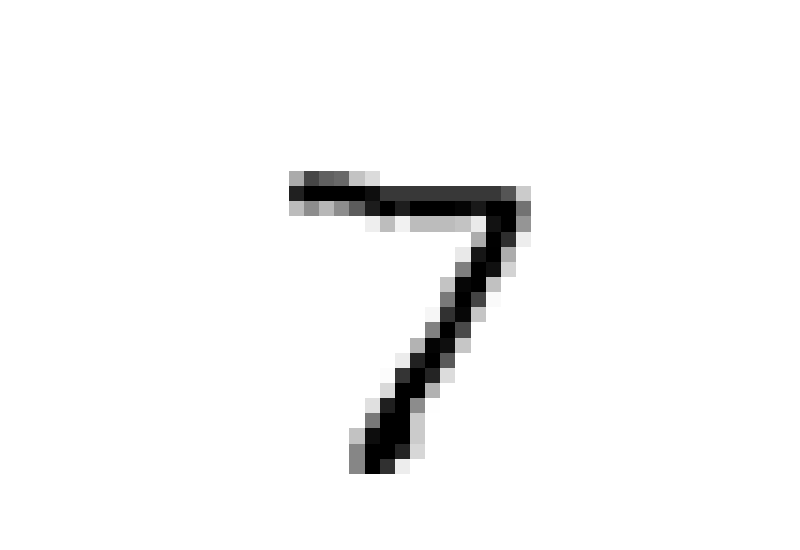
\includegraphics[width=0.5\textwidth]{images/mnist_example}
        \captionof{figure}{MNIST Example}
    \end{center}
\end{multicols}
\end{frame}

% When defining the model, one of the things that we need to define is the layers that our neural network will have.
% We will use an input layer of 784 neurons, as that is the size of our input data.
% We will use a hidden layer of 350 neurons. This size could be changed to optimize the model, or more hidden layers could be added.
% We will use an output layer of 10 neurons, as there are only 10 possible outputs.
\begin{frame}{Defining the Model}{Layers}
    \begin{itemize}
        \item 784 input neurons
        \item 350 hidden neurons
        \item 10 output neurons
    \end{itemize}
\end{frame}

% When defining our model, we also need to define our loss function.
% We will use the mean squared error loss function, shown below, as it simple and still works well.
\begin{frame}{Defining the Model}{Loss Function}
    \begin{itemize}
        \item MSE
        \item $\text{MSE} = \frac{1}{n}\sum_{i=1}^{n}(\hat{y}_i-y_i)^2$
    \end{itemize}
\end{frame}

% The activation function is another important part of the model that needs to be defined.
% We will use the sigmoid activation, shown below, as it is one of the most common and provides a good balance between simplicity and accuracy.
% We also need to define the derivative of the activation function for backpropagation.
\begin{frame}{Defining the Model}{Activation Function}
    \begin{itemize}
        \item Sigmoid
        \item $\sigma(x) = \frac{1}{1+e^{-x}}$
        \item $\sigma'(x) = x(1-x)$
    \end{itemize}
\end{frame}

% To train the model, the data is split into equal sized batches. This saves us from running through the whole dataset multiple times.
% Each batch is then passed through the network, and the loss is calculated.
% This is called an epoch.
% After each epoch, the calculated losses are used to backpropagate through the network and update the weights and biases.
\begin{frame}{Coding a Neural Network}{Training the Model}
\begin{multicols}{2} 
    \begin{itemize}
        \item Split the data into equal sized batches
        \item Forward Propagation for the whole epoch
        \item Backpropagation after each epoch
    \end{itemize}
    \begin{center}
        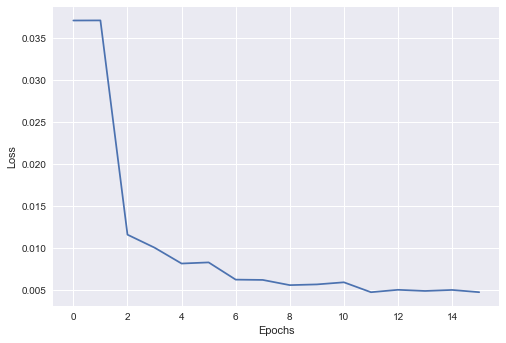
\includegraphics[width=0.5\textwidth]{images/loss}
        \captionof{figure}{Loss over epochs}
    \end{center}
\end{multicols}
\end{frame}

% Once we have a trained model, it is important to test it on unseen data.
% This will give us an idea of how the network might perform in the real world.
% To do this, we will run the test dataset through the model and keep track of how many correct predictions were made.
% Our model has a test accuracy of 99.32%.

\begin{frame}{Coding a Neural Network}{Testing the Model}
    \begin{itemize}
        \item Test the model on unseen data
        \item Run the test dataset through the model
        \item Calculate accuracy by keeping track of how many correct predictions were made
        \item 95.32\% accuracy
    \end{itemize}
\end{frame}

% To get a more visual representation of how our model is performing, 9 images were randomly selected from the test dataset and ran through the model.
% The images are shown below, and had labels of 8, 5, 8,9 1, 9, 7, 2 and 8. 
% The model correctly predicted all but the first one, which it predicted as a 5 instead of an 8.
% This gives an accuracy of 88% on this small batch.
\begin{frame}{Coding a Neural Network}{Testing the Model}
    \begin{multicols}{2} 
        \begin{itemize}
            \item Input labels: 8, 5, 8, 9, 1, 9, 7, 2, 8
            \item predictions: 5, 5, 8, 9, 1, 9, 7, 2, 8
            \item 88\% accuracy
        \end{itemize}
        \begin{center}
            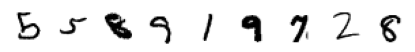
\includegraphics[width=0.5\textwidth]{images/sample_predictions.png}
            \captionof{figure}{Inputs for example predictions}
        \end{center}
    \end{multicols}
\end{frame}

% In conclusion, we have explored what a neural network is, how it works and the steps for how you could code one from scratch.
% Although coding a neural network from scratch has allowed me to learn a lot about them, it is much easier to use a pre-existing library such as tensorflow or pytorch, as they provide a lot more complex models and are very well optimized.
% Thank you for listening.
\begin{frame}{Conclusion}
    \begin{itemize}
        \item Complex models used for many different tasks
        \item Easier and quicker to use a library
        \item I have gained knowledge of neural networks
    \end{itemize}
\end{frame}
\end{document}


